% -----------------------------------------------
% Template for ISMIR Papers
% 2016 version, based on previous ISMIR templates

% Requirements :
% * 6+1 page length maximum
% * 2MB maximum file size
% * Copyright note must appear in the bottom left corner of first page
% (see conference website for additional details)
% -----------------------------------------------

\documentclass{article}
\usepackage{ismir,amsmath,cite}
\usepackage{graphicx}
\usepackage{color}

% ------
\title{Good-sounds.org: a framework to explore goodness in instrumental sounds}

% ------------
\multauthor
{Giuseppe Bandiera$^1$ \hspace{1cm} Oriol Romani Picas$^1$ \hspace{1cm} Hiroshi Tokuda$^2$} { \bfseries{Wataru Hariya$^2$ \hspace{1cm} Koji Oishi$^2$ \hspace{1cm} Xavier Serra$^1$}\\
  $^1$ Music Technology Group, Universitat Pompeu Fabra, Barcelona, Spain\\
$^2$ Technology Development Dept., KORG Inc., Tokyo, Japan\\
{\tt\small giuseppe.bandiera@upf.edu, oriol.romani@upf.edu}
}
\def\authorname{Giuseppe Bandiera, Oriol Romani Picas, Hiroshi Tokuda, Wataru Hariya, Koji Oishi, Xavier Serra}


\sloppy % please retain sloppy command for improved formatting

\begin{document}

%
\maketitle
%
\begin{abstract}
We introduce good-sounds.org, a web framework to explore the concept of goodness in instrumental sounds. The project consists of a database of sounds, music descriptors and annotations about the goodness of the sounds. Both the sounds and the annotations are provided by a community of users. The music descriptors are extracted using the state-of-the-art Music Information Retrieval algorithms available in Essentia’s audio library. The web makes use of modern front-end web technologies to make the user experience seamless and to provide us useful data visualisation tools. Using this framework we performed an experiment to rate goodness on single note sounds of 9 different instruments. We asked the community to perform a task to annotate sounds in a goodness scale. This task is an AB vote according to a set of sound attributes defined in our previous work. With this votes we build a ranking of the sounds for each attribute. A model that rates the goodness in a 0 to 100 score for each sound attribute is built using the rankings and the extracted features.
\end{abstract}
%
\section{Introduction}\label{sec:introduction}

The analysis of sound goodness, or quality, in instrumental sounds is difficult due to its intrinsic subjectivity. Nevertheless, it has been shown that there is some consistency among people while discriminating good or bad music performances \cite{1}. Furthermore, recent studies have demonstrated a correlation between the perceived music quality and the musical performance technique \cite{2}. Bearing this in mind, in a previous work \cite{01} we tried to automatically rate goodness by defining a set of sound attributes and by using a set of good/bad labels given by  expert musicians. The definition of goodness was treated as a classification problem and an outcome of that work was a mobile application (Cortosia) that gives a goodness score of single notes in real-time on a scale from 0 to 100. This score was computed considering the distribution of the features values in the classification step. During the process of developing the system we realised that we could improve the scores, specially their correlation with the perceptual sound goodness, if we could use more training data, specially including a range of goodness levels given by users rather than binary good/bad labels. However, the task of labeling sounds this way is very time consuming and we would need sounds with which to cover the whole range of sound goodness. To address these issues we developed a website, good-sounds.org, on which users could upload sound content and the appropriate metadata to explore a richer view of sound goodness.     
%
\section{good-sounds.org}\label{sec:goodsounds}
Good-sounds.org\footnote{\textit{https://good-sounds.org/}} is a web platform to explore the concept of goodness in instrumental sounds with the help of a community of users. The website provides social community features in the front end and a framework for sound analysis and modeling in the background. It also includes an easy access to most some its features through an API.

\subsection{Description} 
The website has been designed from a user perspective,  meant to be modern and to provide a seamless experience. It makes use of state of the art designing concepts and community oriented web technologies. The front end includes three main sections: (1) a visualisation page of the sounds that is shown in the home page if user is authenticated, (2) an upload section and (3) an annotation task. The visualisation page shows a list of all the sounds in the database that can be filtered by several options like instrument or uploading date. The upload page allows the users to add or drag several sounds and also provides a recording tool built using Web Audio API\footnote{\textit{http://www.w3.org/TR/webaudio/}}. The annotation page is by now designed for the specific experiment we will explain in section 3. 
The website backend is written in Python using the Django web application framework. The metadata is stored in a PostgreSQL database while the files are stored locally in the server. An API accepts requests from authorized clients to upload sounds and retrieve statistics from the user’s community. 
At this time the community consists of 363 active users. The website supports 11 instruments and has 8470 unique sounds

\subsection{Content}
The data stored in good-sounds.org consists of audio and metadata. The audio is first processed using the freesound extractor \cite{02} to get an mp3 version of the audio and images for the waveform and the spectrogram. These files are stored in the good-sounds server. All the metadata is stored in the PostgreSQL database. The users can decide on three different types of Creative Commons licenses for their content: Universal, Attribution or Attribution Non-Commercial. 
In addition to the content described previously, the website contains music information retrieval data such as music descriptors, features and segmentation training data.

\subsubsection{Segmentation}
One of the critical sections of the music analysis framework in good-sounds.org is a set of algorithms to segment the audio into notes. As the audio come from different sources they can have several issues (silence at the end, background noise..) that difficult the subsequent feature extraction step. 
To perform this segmentation we use the state of the art music information retrieval algorithms available in the open source Essentia library \cite{03}. Considering that the sounds we are working with are all monophonic pitched instrument sounds we base the segmentation on pitch . Our approach extracts pitch using two different algorithms: the Essentia’s implementations of the YinFFT algorithm \cite{04} and the Yin time based algorithm \cite{05}. Then we finally segment the sound into notes using pitch contours \cite{06} and signal RMS with Essentia’s PitchContourSegmentation algorithm.  
All the data related to segmentation is stored in the good-sounds.org database. This allows us to build client-side data visualizations that effectively reflect the quality of the segmentation algorithm. Moreover, the user can input new parameters for this algorithm and re-run it on the fly from the website: the results of this iteration will immediately be shown on the same page, for an easy comparison of the results.

\subsubsection{Descriptors}
The feature extraction module computes spectral, tonal and temporal descriptors. Most of them are described in \cite{07}. The audios are resampled to 44.1kHz sampling rate and normalised using replay gain. The descriptors are then extracted across all the frames using a 2048 window size and 512 hop window size. We then compute statistical measures of this descriptors that are stored in JSON files in the server. A list of the descriptors we extract is shown in Table~\ref{table:descriptors}. As statistical measures we use mean, median and standard deviation. 

\begin{table*}[ht]
\centering
\begin{tabular}{lll}
\hline
spectral                                                                                                                                                                                 & tonal                                      & temporal                                            \\ \hline
\begin{tabular}[c]{@{}l@{}}spectrum, barkbands, \\ melbands, flatness, crest, rolloff, \\ decrease, hfc, pitch salience, flatness db, \\skewness, kurtosis, spectral complexity,\end{tabular} & pitch yinfft, pitch yin, pitch confidence, & zerocrossingrate, loudness, centroid, \\flatness sfx, \\
\hline
\end{tabular}
\caption{Descriptors extracted by Essentia library present in good-sounds.org}
\label{table:descriptors}
\end{table*}


\section{Experiment} \label{experiment}
As a test case for the good-sounds.org framework we setup an experiment to rate the goodness of single notes. We make use of the dataset we collected in our previous work and we take advantage of the community to annotate this dataset through a voting task. We also take into account the annotations made by music experts in the recording process. The goal of the experiment is to build models with the community annotations for automatically rating the sound goodness of single notes. We then compare this models to the ones built in our previous work using the expert annotations.  

\subsection{Dataset}
The data used in this experiment comes from several different sources. First, we uploaded all the sounds from our previous work to the website, as well as their expert annotations. The sounds coming from the mobile app through the API and the ones uploaded to website by the community are also considered. Finally, annotations on the sounds according to a goodness scale are collected using a voting task. 
This annotations are taken according to a set of sound attributes that affect sound goodness. We defined this attributes in our previous work together with a group of music experts:   
\begin{itemize}
	\item{\textit{dynamic stability}: the stability of the loudness.}
	\item{\textit{pitch stability}: the stability of the pitch.}
	\item{\textit{timbre stability}: the stability of the timbre.}
	\item{\textit{timbre richness}: the quality of the timbre.}
	\item{\textit{attack clarity}: the quality of the attack.}
\end{itemize}

\subsubsection{Sounds}
For this experiment we selected only the single note sounds. At this time there are in the good-sounds database 5467 single note of 9 instruments. We show the list of sounds per instrument in Table~\ref{sounds}. The sounds from the recording sessions are uncompressed wave files while the ones uploaded to the website by community users can have several different audio formats.  

\begin{table}[ht]
\centering
\begin{tabular}{cc}
\hline
instrument   & number of sounds \\ \hline
cello        & 935              \\
violin       & 802              \\
clarinet     & 1360             \\
flute        & 1434             \\
alto sax     & 352              \\
baritone sax & 292              \\
tenor sax    & 292              \\
soprano sax  & 343              \\
trumpet      & 738              \\ \hline
\end{tabular}
\caption{Number of sounds in the exepriment's dataset}
\label{sounds}
\end{table}

\subsubsection{Annotations}
We distinguish two kind of annotations that we call recording annotations and community annotations. The first annotations are the ones coming from the recording sessions and consists of one tag per sound. This tag express if the sound is a good or a bad example of each sound attribute (e.g. bad-timbre-stability, good-attack-clarity…). Those are the annotations used later on for a first evaluation of the models and are only available for the sounds we recorded ourselves.
The second class of annotations are the ones used in this work to explore goodness. In order to be able to rate a sound in a goodness scale we need annotations on a wide range of different goodness levels. We discarded asking the community to rate sounds in a scale of goodness because of the following:

\begin{itemize}
	\item{the task can be excessively demanding.}
	\item{without a reference sound the criteria of different users can differ extremely.}
	\item{with a reference sound we influence the user’s criteria, thus annotations can be less 	generalisable.}
\end{itemize}

To solve this we designed a task to sort the sounds in a ranking of goodness for each sound attribute. An A/B multi vote task is used for this purpose. Two sounds are presented and the user is asked to decide which sound is better according to one or more of the sound attributes. On vote is stored for each selected attribute. A list of the votes per instruments (considering all sound attributes) is shown in Table~\ref{votes}.
In order to prevent random votes in the task we run checks periodically. This checks consists of two sounds; one being a bad example of a sound attribute regarding the expert annotations and the other being a good example. The task is presented to the users the first time they vote and also randomly after some votes. If the user does not vote for the sound is expected in the reference task, his next votes are not considered. The votes of this user are again taken into account if he succeeds on the reference task. 


\begin{table}[ht]
\centering
\begin{tabular}{cc}
\hline
instrument   & number of votes \\ \hline
cello        & 140             \\
violin       & 90              \\
clarinet     & 293             \\
flute        & 305             \\
alto sax     & 78              \\
baritone sax & 59              \\
tenor sax    & 14              \\
soprano sax  & 21              \\
trumpet      & 230             \\ \hline
\end{tabular}
\caption{Number of votes in good-sounds for the dataset's experiment.}
\label{votes}
\end{table}

\subsubsection{Rankings}
In order to have learning data in a wide range of goodness we build rankings with the community votes for each sound attribute. The position of a sound in the ranking represents its goodness level. To build them we count the number of wins and the number of votes of each sound in the database. Then the sounds are sorted according to two parameters; 

\begin{itemize}
	\item{total number of votes: number of participations in the voting task.}
	\item{ratio between wins and votes: the ratio between the number of wins and the total number of participations in the voting task.}
\end{itemize}
  
Using this parameters for building the rankings we assess that the sounds in the top are the ones voted many times as being better than others and not sounds with few votes but high percentage of wins.

\subsection{Learning}
The goal of our learning process is to build a model for each instrument that is able to rate each sound attribute in a 0 to 100 score. To do so we want to find a set of features that highly correlate with the rankings extracted in the previous step.  
Our approach uses a regression model to predict the score. These predictions are then used as samples of the final score function. The final score is then computed as an interpolation of the samples.

\subsubsection{Models}
We want to find the combination of regression model and set of features that better describes the rankings. For such a purpose we use all the different regression algorithms available in scikit-learn \cite{08}.  For each one of the algorithms we build a model for each ranking using one, two or three features and we compute the average prediction score of the model across all the options. The prediction score $R^2$ is defined in the scikit-learn documentation as follows:

\begin{equation}
 R^2 = (1 - u/v) 
\end{equation}
where
\begin{equation}
	u = \sum\nolimits((y_{true} - y_{pred})^2)
\end{equation}
and
\begin{equation}
	v = \sum\nolimits((y_{true} - \prod\limits_{i=1}^n y_{true})^2)
\end{equation}

Where $y_{true}$ is the set of ground truth annotations and $y_{pred}$ the set of predictions, having both the same length. The best possible score $R^2$ is 1.0 and it can be negative.
The variance of the prediction score across all the rankings and set of features is also computed. 
The number of features that give the best score for each ranking is taken into account to compute an average number of features for each regression model. A comparison of the performance of the different models is shown in Table~\ref{models}.

\begin{table*}[]
\centering
\label{my-label}
\begin{tabular}{cccc}
\hline
Regression model  & Avg. score & Score variance & Average of features \\ \hline
SVR               & -1.208     & 5.4436         & 1.843               \\
Ridge             & -2.644     & 31.005         & 2.166               \\
KRR               & -1.79      & 10.798         & 1.906               \\
Linear regression & -3.503     & 30.03          & 1.718               \\
RANSAC            & -3.202     & 17.532         & 1.478               \\
Theilsen          & -4.14      & 37.135         & 1.781               \\ \hline
\end{tabular}
\caption{Performance of the different regression models}
\label{models}
\end{table*}

As we can see in the table the SVR (Epsilon-Support Vector Regression) model has the best average score across all the rankings and using all possible combination of feature sets (up to 3 features). It also has the lowest score variance so we can expect the model to be robust across the different instruments and sound attributes. Even so, the average number of features is almost two. The computation of two features for each frame of all the sounds in the database can be expensive for the server. For this reason we want to know how good the model can be if we force it to use less than three features. We show the results of such a comparison in Table~\ref{svr}.

\begin{table}[]
\centering
\label{my-label}
\begin{tabular}{lll}
\hline
Regression model & Avg. score & Score variance \\ \hline
SVR 3 features   & -1.208     & 5.4436         \\
SVR 2 features   & -1.2411    & 5.3895         \\
SVR 1 feature    & -1.4254    & 5.6554         \\ \hline
\end{tabular}
\caption{Performance of SVR model with differnet number of features.}
\label{svr}
\end{table}

The results show that the use of more than one feature is not significantly an advantage so we decide to use SVR with a single feature. We then try all the possible combinations of parameters (kernel, degree of polinomiality, cost parameter..) to find the best model for each instrument and sound attribute.

\subsubsection{Scores}
Once the model is build it is able to predict the ranking position of a sound. We then map this position into a 0 to 100 score of the sound attribute. The final goodness score is computed as the average score across the five attributes. We compute the sound attribute scores of all the sounds in the database to test the distribution of the scores according to the feature value. A distribution of the score for the timbre stability of flute is shown in Figure~\ref{fig:scores}.

\begin{figure}[ht]
 \centerline{\framebox{
 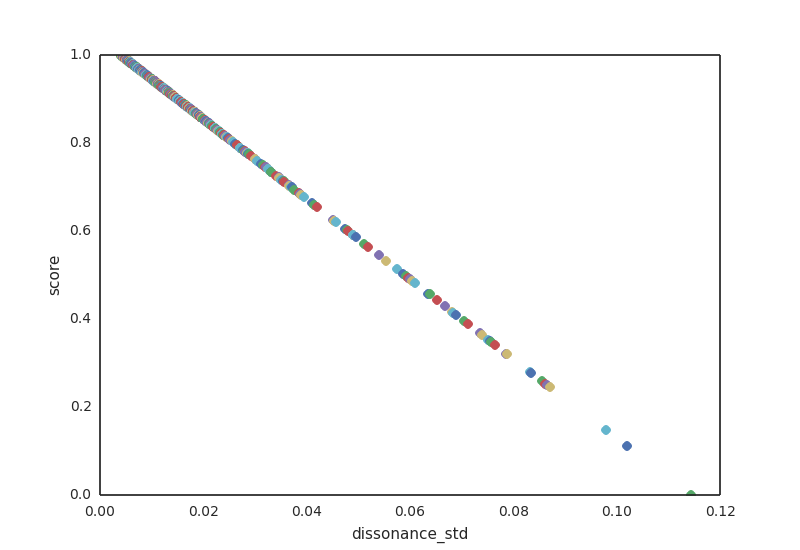
\includegraphics[width=\columnwidth]{figs/distribution_1.png}}}
 \caption{Distribution of scores of flute timbre stability.}
 \label{fig:scores}
\end{figure}

All these distributions are not balanced. For this reason we push the scores of each sound attribute to fit a Gaussian distribution. This allow us to refine the scores by tweaking the parameters of the gaussian function and in addition the distribution of the scores is balanced.
A result of this process is shown in Figure~\ref{fig:scores_2}. The final score is computed interpolating the feature according to these tuned distributions. 

\begin{figure}[ht]
 \centerline{\framebox{
 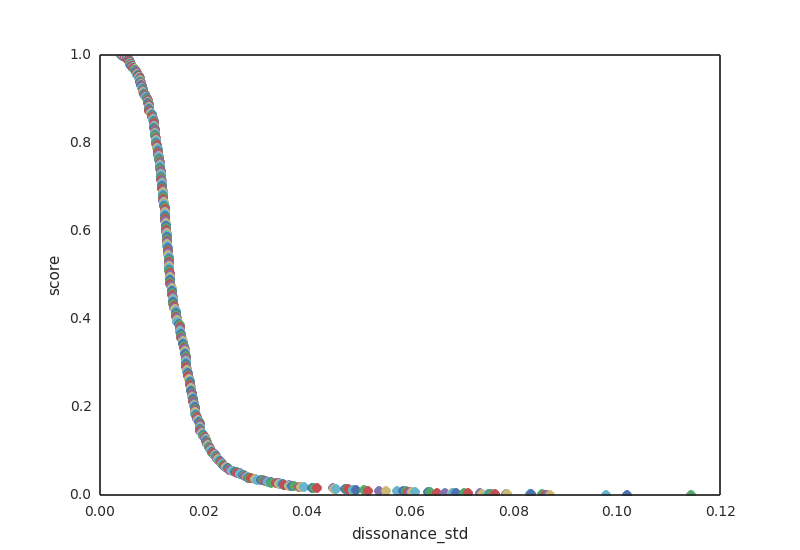
\includegraphics[width=\columnwidth]{figs/distribution_2.png}}}
 \caption{Distribution of scores of flute timbre stability after normalisation.}
 \label{fig:scores_2}
\end{figure}

\subsubsection{Models evaluation}
In order to evaluate if the scores provided by the models fit the perceived goodness we first take advantage of the expert annotations of our previous work. Not all the sounds from which we have expert annotations have community votes thus are useful for evaluation. The scores of all this sounds are computed using the models. We use the data visualisation tools implemented in the website to visualise these scores according to the expert annotations. This tools allows us to easily understand how the models perform. An example of flute timbre stability scores according to the expert annotations is shown in Figure~\ref{fig:scores}.

\begin{figure}
 \centerline{\framebox{
 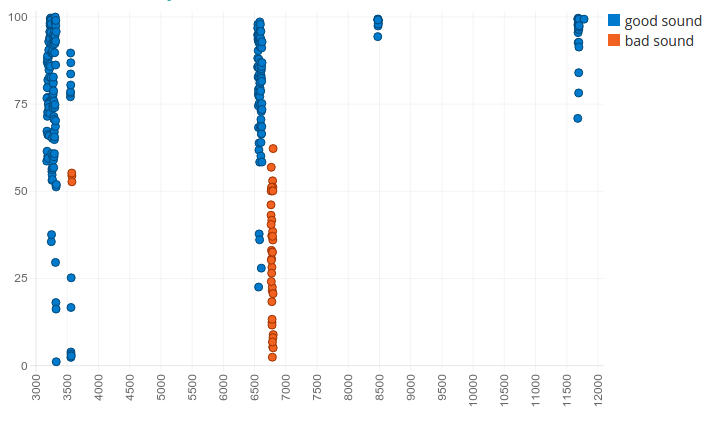
\includegraphics[width=\columnwidth]{figs/scores.png}}}
 \caption{Visualisation of scores through the website}
 \label{fig:scores_3}
\end{figure}

Through this tool we can see that the scores tend to be below 50 for bad sound examples and above 50 for good examples. The scores for all the sounds in the database having expert annotations are analysed. Table~\ref{results} shows the number of sounds per sound attribute with scores above and below 50 according to their tags.

\begin{table}[ht]
\centering
\begin{tabular}{lll}

             & Dynamics stability     &                    \\ \hline
sound tag    & score \textgreater= 50 & score \textless 50 \\ \hline
good sound   & 1846                   & 872                \\
bad dynamics & 438                    & 881                \\
             &                        &                    \\

             & Timbre stability       &                    \\ \hline
sound tag    & score \textgreater= 50 & score \textless 50 \\ \hline
good sound   & 930                    & 429                \\
bad timbre   & 224                    & 472                \\
             &                        &                    \\

             & Pitch stability        &                    \\ \hline
sound tag    & score \textgreater= 50 & score \textless 50 \\ \hline
good sound   & 1260                   & 99                 \\
bad pitch    & 125                    & 636                \\
			 &                        &                    \\

             & Timbre richness        &                    \\ \hline
sound tag    & score \textgreater= 50 & score \textless 50 \\ \hline
good sound   & 1184                   & 175                \\
bad richness & 380                    & 268                \\
             &                        &                    \\

             & Attack clarity         &                    \\ \hline
sound tag    & score \textgreater= 50 & score \textless 50 \\
good sound   & 1005                   & 354                \\
bad attack   & 553                    & 294                \\ \hline
\end{tabular}
\caption{Number of sounds for each sound attribute with scores higher or lower than 50.}
\label{results}
\end{table}

As we can see the models seem to perform better in rating good sound examples. If we consider as correct predictions the sounds with “good sound” tag and score above 50 as well as the ones having “bad attribute” tag and score below 50 there are 8778 correct predictions out of 12427. 

\section{Conclusions}
We presented a web based framework for exploring sound goodness in instrumental sounds through a community of users. The framework provides an easy way to collect sounds and annotations as well as tools to extract and store music descriptors. This allows us to explore the concept of sound goodness in a controlled and flexible environment. Furthermore, it is useful for the community as a place in which to discuss the issues affecting sound goodness as well as a learning tool to improve their playing techniques. 
As a test case for the framework we extended the work presented in [1] by using annotations from the community collected through a voting task. The models built using this approach provide an automatic rating of goodness for each attribute that tends to match the expert annotations collected in our previous work. The results should improve with more annotations from the community.
As future work we want to design new tasks to collect user annotations and build new models according to them.or designing a different task to collect these annotations. 

\section{Acknowledgements}
This research has been partially funded by KORG Inc. The authors would like to thank the entire good-sounds.org community who contributed to the website with sounds and annotations.

% For bibtex users:
%\bibliography{ISMIRtemplate}

% For non bibtex users:
\begin{thebibliography}{citations}
%
\bibitem {1}
J. Geringer and C. Madsen
``Musicians ratings of good versus bad vocal and string performances''
{\it Journal of Research in Music Education}, vol. 46, pages 522-34, 1998.

\bibitem {2}
Brian E. Russell
``An empirical study of a solo performance assessment model''
{\it  International Journal of Music Education}, vol. 33, pages 359-371, 2015.

\bibitem {01}
O. Romani Picas et al.
``A real-time system for measuring sound goodness in instrumental sounds,''
{\it AES 138th Convention Warsaw}, 2015.

\bibitem {02}
 F. Font, G. Roma, and X. Serra
``Freesound technical demo,''
{\it Proceedings of the 21st ACM international conference on Multimedia.}, 2013.

\bibitem {03}
 D. Bogdanov et al.
``Essentia: An audio analysis library for music information retrieval,''
{\it  In Proceedings of the International Society for Music Information Retrieval Conference.}pages 493–498, 2013.

\bibitem {04}
 P. M. Brossier
``Automatic Annotation of Musical Audio for Interactive Applications''
{\it QMUL, London, UK,}, 2007.

\bibitem {05}
 A. de Cheveigné and H. Kawahara.
``YIN, a fundamental frequency estimator for speech and music''
{\it The Journal of the Acoustical Society of America}111:1917, 2002.

\bibitem {06}
 R. J. McNab et al.
``Signal processing for melody transcription''
{\it In Proceedings of the 19th Australasian Computer Science Conference}, 1996.

\bibitem {07}
P. M. Brossier.
``Automatic Annotation of Musical Audio for Interactive Applications''
{\it Ph.D. Thesis, Queen Mary University of London, UK}, 2007.

\bibitem {08}
Pedregosa et al.
``Scikit-learn: Machine Learning in Python''
{\it JMLR 12}, pages. 2825-2830, 2011.


\end{thebibliography}

\end{document}
